\documentclass[11pt,letterpaper]{article}
\usepackage[margin=0.85in,headheight=14pt]{geometry}
\usepackage{amsmath,amssymb}
\usepackage{enumitem}
\usepackage{fancyhdr}
\usepackage{lmodern}
\usepackage[T1]{fontenc}
\usepackage[dvipsnames]{xcolor}
\usepackage[most]{tcolorbox}
\usepackage{pgfplots}
\usepgfplotslibrary{groupplots}
\usetikzlibrary{arrows.meta,positioning,shapes.geometric,calc,decorations.markings}
\pgfplotsset{
  compat=1.18,
  every axis/.append style={grid=major, grid style={gray!25}, tick label style={font=\footnotesize},
    label style={font=\small}, title style={font=\small}, legend style={font=\scriptsize}},
}
\definecolor{cA}{HTML}{1F77B4}
\definecolor{cB}{HTML}{FF7F0E}
\definecolor{cC}{HTML}{2CA02C}
\definecolor{cD}{HTML}{D62728}
\definecolor{cE}{HTML}{9467BD}

\pagestyle{fancy}
\fancyhf{}
\lhead{SYDE 556/750 \qquad Practice Test 3C}
\rhead{Solutions \& marking guide}
\cfoot{\thepage}
\renewcommand{\headrulewidth}{0pt}

\setlength{\parindent}{0pt}
\setlength{\parskip}{4pt}

\newcommand{\tin}{\tau_{\mathrm{in}}}
\newcommand{\ans}[1]{\par\vspace{4pt}{\bfseries #1}\quad}

\newtcolorbox{marking}{colback=blue!3,colframe=blue!40!black,boxrule=0.4pt,left=4pt,right=4pt,top=2pt,bottom=2pt,arc=1pt,fonttitle=\bfseries\small,title=Marking}
\newtcolorbox{trap}{colback=red!4,colframe=red!50!black,boxrule=0.4pt,left=4pt,right=4pt,top=2pt,bottom=2pt,arc=1pt,fonttitle=\bfseries\small,title=Where marks are usually lost}

\begin{document}

\begin{center}
{\Large\bfseries Practice Test 3C: Nengo \& Simple Dynamics --- Solutions}\\[2pt]
Total: 20 marks plus 2 bonus. Curves that come from a simulation use \texttt{pn3\_data/make\_data\_3c.py}.\\
Tuning curves use $\tau_{\mathrm{ref}} = 2$ ms and $\tau_{RC} = 20$ ms. Any LIF shape with the labelled intercepts earns the mark.
\end{center}

%=====================================================================
\section*{Question 1 \hfill (4)}

\ans{(a) [2]}
Nengo stores the intercept as a fraction of the radius, and defines the maximum rate as the rate at $\langle e, x\rangle = R$. Scaling the radius stretches the tuning curve by that same factor: $a_{2R}(x) = a_R(x/2)$.
\begin{itemize}[leftmargin=1.2em]
\item \textbf{Radius 1.} Firing starts at $x = 0.25$. The rate is $100$ Hz at $x = 1$. Past the radius the current keeps growing, so the rate keeps rising (about $170$ Hz at $x = 2$ with the time constants above). It does not fall back to zero.
\item \textbf{Radius 2.} The same normalized intercept is now at $x = 0.5$, and $100$ Hz is reached at $x = 2$. The curve is the radius-$1$ curve stretched horizontally by $2$.
\end{itemize}
\begin{center}
\begin{tikzpicture}
\begin{axis}[width=0.78\textwidth, height=5.6cm, xmin=-2, xmax=2, ymin=0, ymax=200,
  xlabel={$x$}, ylabel={firing rate (Hz)}, legend pos=north west, legend cell align=left]
  \addplot[cA, very thick] table[x=x, y=r1] {pn3_data/q1_radius.dat};
  \addplot[cD, very thick] table[x=x, y=r2] {pn3_data/q1_radius.dat};
  \legend{{radius $1$}, {radius $2$}}
  \draw[cA, dashed] (axis cs:0.25,0) -- (axis cs:0.25,40);
  \draw[cD, dashed] (axis cs:0.5,0) -- (axis cs:0.5,40);
  \draw[gray, dotted] (axis cs:1,0) -- (axis cs:1,100) -- (axis cs:-2,100);
  \node[font=\scriptsize, anchor=west] at (axis cs:0.28,55) {start at $0.25$};
  \node[font=\scriptsize, anchor=west] at (axis cs:0.55,28) {start at $0.5$};
  \node[font=\scriptsize, anchor=south west] at (axis cs:1.05,100) {$100$ Hz at $x = R$};
\end{axis}
\end{tikzpicture}
\end{center}
\begin{marking}
0.5: radius $1$ starts at $0.25$ and is at $100$ Hz at $x = 1$. \ 0.5: radius $2$ starts at $0.5$ and is at $100$ Hz at $x = 2$. \ 0.5: the radius-$2$ curve is the wider one. \ 0.5: past its $100$ Hz point the radius-$1$ curve is still high.
\end{marking}
\begin{trap}
Drawing the larger radius as a steeper curve, or dropping the rate to zero once $x$ passes the radius. A bigger radius spreads the same curve over a wider interval.
\end{trap}

\ans{(b) [2]}
The neuron sees $\langle e, \mathbf x\rangle / R$. Along $\mathbf x = (s, 0)$ with $e = (-1, 0)$ and $R = 3$, that is $-s/3$. It starts firing when $-s/3 = 1/3$, i.e.\ at $s = -1$, and it reaches $90$ Hz when $-s/3 = 1$, i.e.\ at $s = -3$. For every $s > -1$ it is silent. The curve rises as $s$ decreases.
\begin{center}
\begin{tikzpicture}
\begin{axis}[width=0.72\textwidth, height=5.2cm, xmin=-3, xmax=3, ymin=0, ymax=110,
  xlabel={$s$}, ylabel={firing rate (Hz)}, title={along $(s, 0)$, encoder pointing left}]
  \addplot[cA, very thick] table[x=s, y=rate] {pn3_data/q1_encoder.dat};
  \draw[gray, dashed] (axis cs:-1,0) -- (axis cs:-1,70);
  \node[font=\scriptsize, anchor=west] at (axis cs:-0.9,74) {starts at $s = -1$};
  \node[font=\scriptsize, anchor=west] at (axis cs:-2.95,96) {$90$ Hz};
\end{axis}
\end{tikzpicture}
\end{center}
\begin{marking}
1: zero to the right of $s = -1$, and firing starts at $s = -1$. \ 1: the rate grows as $s$ decreases and reaches $90$ Hz at $s = -3$.
\end{marking}
\begin{trap}
A tuning curve that rises to the right. This encoder points in the negative direction, so the neuron prefers negative $s$.
\end{trap}

%=====================================================================
\section*{Question 2 \hfill (4)}

\ans{(a) [2]}
The target is $\dot x = Ax + Bv$ with $A = -1/5$ and $B = 1$. With $\tau = 0.1$,
\[
A' = \tau A + 1 = 1 - \frac{0.1}{5} = \mathbf{0.98}, \qquad B' = \tau B = \mathbf{0.1}.
\]
With $v = 0$ the system is $\dot x = -x/5$, so
\[
x(t) = 0.4\,e^{-t/5}, \qquad x(5) = 0.4/e \approx \mathbf{0.147}.
\]
The effective time constant is $\tau/(1 - A') = 0.1/0.02 = 5$ s, which is the $5$ in the target system. The synapse is $0.1$ s; the feedback cancels most of its leak and leaves a $5$ s memory.
\begin{center}
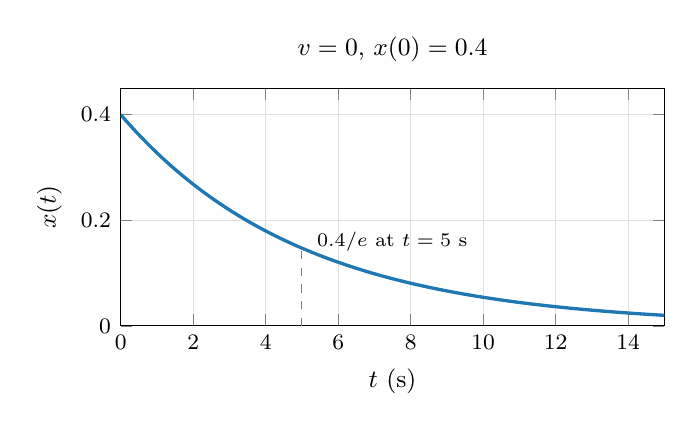
\begin{tikzpicture}
\begin{axis}[width=0.7\textwidth, height=4.6cm, xmin=0, xmax=15, ymin=0, ymax=0.45,
  xlabel={$t$ (s)}, ylabel={$x(t)$}, title={$v = 0$, $x(0) = 0.4$}]
  \addplot[cA, very thick, domain=0:15, samples=100] {0.4*exp(-x/5)};
  \draw[gray, dashed] (axis cs:5,0) -- (axis cs:5,0.147);
  \node[font=\scriptsize, anchor=west] at (axis cs:5.15,0.16) {$0.4/e$ at $t = 5$ s};
\end{axis}
\end{tikzpicture}
\end{center}
\begin{marking}
0.5: $A' = 0.98$. \ 0.5: $B' = 0.1$. \ 0.5: $x(t) = 0.4e^{-t/5}$. \ 0.5: $x(5) = 0.4/e$ (a value from $0.14$ to $0.15$ is fine).
\end{marking}

\ans{(b) [2]}
Now $A = -20$ and $B = 20$:
\[
A' = 0.1(-20) + 1 = \mathbf{-1}, \qquad B' = 0.1(20) = \mathbf{2}.
\]
A unit step settles at $x = u = 1$. The network time constant is $\tau/(1 - A') = 0.1/2 = \mathbf{0.05}$ \textbf{s}, so
\[
x(t) = 1 - e^{-20t}.
\]
The synapse alone is $1 - e^{-t/0.1} = 1 - e^{-10t}$, which is slower. Negative feedback adds to the leak instead of cancelling it, and the large input transform $B' = 2$ keeps the steady state at $1$. The loop can be faster than the synapse it is built from.
\begin{center}
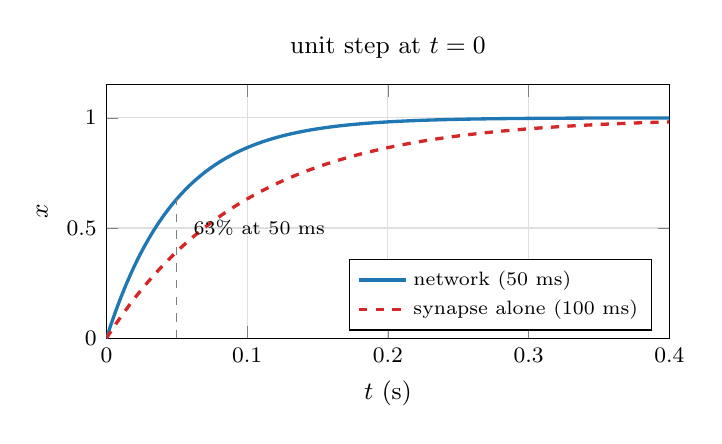
\begin{tikzpicture}
\begin{axis}[width=0.72\textwidth, height=4.8cm, xmin=0, xmax=0.4, ymin=0, ymax=1.15,
  xlabel={$t$ (s)}, ylabel={$x$}, legend pos=south east, legend cell align=left,
  title={unit step at $t = 0$}]
  \addplot[cA, very thick, domain=0:0.4, samples=120] {1 - exp(-20*x)};
  \addplot[cD, very thick, dashed, domain=0:0.4, samples=120] {1 - exp(-10*x)};
  \legend{{network ($50$ ms)}, {synapse alone ($100$ ms)}}
  \draw[gray, dashed] (axis cs:0.05,0) -- (axis cs:0.05,0.63);
  \node[font=\scriptsize, anchor=west] at (axis cs:0.055,0.5) {$63\%$ at $50$ ms};
\end{axis}
\end{tikzpicture}
\end{center}
\begin{marking}
0.5 each: $A' = -1$, $B' = 2$. \ 0.5: both curves go to $1$, and the network reaches it sooner (time constant $50$ ms). \ 0.5: the network is faster because $A' < 1$ strengthens the leak ($A' = -1$ here).
\end{marking}
\begin{trap}
Putting the $50$ ms on the synapse. The synapse stays at $0.1$ s. Also, $A' = \tau A$ without the $+1$ gives $-2$ instead of $-1$.
\end{trap}

%=====================================================================
\section*{Question 3 \hfill (4)}

\ans{(a) [2]}
\[
\tau\dot x = 0 + x^3 - x = \boxed{\,x^3 - x\,} = x(x - 1)(x + 1).
\]
Equilibria at $x = -1,\ 0,\ 1$. The slope is $\varphi'(x) = 3x^2 - 1$:
\begin{itemize}[leftmargin=1.2em]
\item $x = 0$: $\varphi' = -1 < 0$, \textbf{stable}. Between $-1$ and $1$, $\varphi$ pushes back toward $0$.
\item $x = \pm 1$: $\varphi' = 2 > 0$, \textbf{unstable}. Outside that interval $\varphi$ has the same sign as $x$, so the state runs away.
\end{itemize}
\begin{marking}
1: $\varphi(x) = x^3 - x$, with the synapse's $-x$ included. \ 0.5: all three equilibria. \ 0.5: $0$ stable and $\pm 1$ unstable, with a reason.
\end{marking}
\begin{trap}
Dropping the $-x$, which leaves only the equilibrium at $0$ and makes it unstable. The cubic $x - x^3$ has the opposite stability: there the outer points are the stable ones.
\end{trap}

\ans{(b) [2]}
\begin{itemize}[leftmargin=1.2em]
\item $x(0) = 0.5$ is between the unstable points, and $\varphi(0.5) < 0$, so $x$ decreases and settles at $\mathbf{0}$.
\item $x(0) = 1.2$ is past the unstable point at $1$. $\varphi(1.2) > 0$, so $x$ increases until the population saturates at the radius, $\mathbf{+2}$.
\end{itemize}
The trajectories below use $\tau = 0.1$ s and stop at the radius.
\begin{center}
\begin{tikzpicture}
\begin{groupplot}[group style={group size=2 by 1, horizontal sep=1.5cm}, height=5.4cm]
\nextgroupplot[width=0.48\textwidth, xmin=-2, xmax=2, ymin=-1.5, ymax=6,
  xlabel={$x$}, ylabel={$\varphi(x) = x^3 - x$}, title={phase portrait}]
  \addplot[cA, very thick] table[x=x, y=phi] {pn3_data/q3_phi.dat};
  \addplot[black, thin, domain=-2:2, samples=2] {0};
  \addplot[only marks, mark=*, mark size=2.5pt, black] coordinates {(0,0)};
  \addplot[only marks, mark=o, mark size=2.5pt, thick, black] coordinates {(-1,0) (1,0)};
  \draw[-{Stealth}, very thick, cD] (axis cs:-1.7,0.35) -- (axis cs:-1.95,0.35);
  \draw[-{Stealth}, very thick, cD] (axis cs:-0.7,0.35) -- (axis cs:-0.15,0.35);
  \draw[-{Stealth}, very thick, cD] (axis cs:0.7,0.35) -- (axis cs:0.15,0.35);
  \draw[-{Stealth}, very thick, cD] (axis cs:1.7,0.35) -- (axis cs:1.95,0.35);
  \node[font=\scriptsize, anchor=south] at (axis cs:0,0.55) {stable};
  \node[font=\scriptsize, anchor=south] at (axis cs:1,0.7) {unstable};
  \node[font=\scriptsize, anchor=south] at (axis cs:-1,0.7) {unstable};
\nextgroupplot[width=0.5\textwidth, xmin=0, xmax=0.8, ymin=-2.15, ymax=2.15,
  xlabel={$t$ (s)}, ylabel={$x(t)$}, title={$\tau = 0.1$ s, radius $2$},
  legend style={at={(0.5,-0.32)}, anchor=north}, legend cell align=left]
  \addplot[cA, very thick] table[x=t, y=a] {pn3_data/q3_traj.dat};
  \addplot[cB, very thick] table[x=t, y=b] {pn3_data/q3_traj.dat};
  \addplot[cE, very thick, dashed] table[x=t, y=c] {pn3_data/q3_traj.dat};
  \legend{{$x(0) = 0.5$}, {$x(0) = 1.2$}, {$x(0) = -1.2$}}
\end{groupplot}
\end{tikzpicture}
\end{center}
The third curve is the mirror of the second: $x(0) = -1.2$ saturates at $-2$. It is not asked, but it is the same rule.
\begin{marking}
0.5: sketch with $\varphi(0) = 0$ stable and crossings at $\pm 1$ unstable, arrows inward between them and outward outside. \ 0.5: $x(0) = 0.5$ goes to $0$. \ 1: $x(0) = 1.2$ runs away to the positive saturation.
\end{marking}

%=====================================================================
\section*{Question 4 \hfill (4)}

\ans{(a) [1]}
$\tau\omega = 0.05\pi = \pi/20$:
\[
A' = \begin{bmatrix} 1 & -\pi/20 \\ \pi/20 & 1 \end{bmatrix}
\approx \begin{bmatrix} 1 & -0.157 \\ 0.157 & 1 \end{bmatrix}.
\]
\begin{marking}
0.5: ones on the diagonal. \ 0.5: off-diagonal entries $\mp\pi/20$ with the same sign pattern as $A$.
\end{marking}

\ans{(b) [3]}
Rotating the initial state by the angle $\omega t = \pi t$ gives
\[
\begin{aligned}
x_1(t) &= 0.6\cos(\pi t) - 0.8\sin(\pi t),\\
x_2(t) &= 0.6\sin(\pi t) + 0.8\cos(\pi t).
\end{aligned}
\]
Since $0.6^2 + 0.8^2 = 1$, both signals have amplitude $1$. The period is $2\pi/\omega = \mathbf{2}$ \textbf{s}, so the window is one cycle. Equivalently $x_1 = \cos(\pi t + \phi)$ and $x_2 = \sin(\pi t + \phi)$ with $\cos\phi = 0.6$ and $\sin\phi = 0.8$.

At $t = 0$ the state is $(0.6, 0.8)$. There $\dot x_1 = -\omega x_2 < 0$ and $\dot x_2 = \omega x_1 > 0$, so it moves left and up: \textbf{counter-clockwise} around the unit circle.
\begin{center}
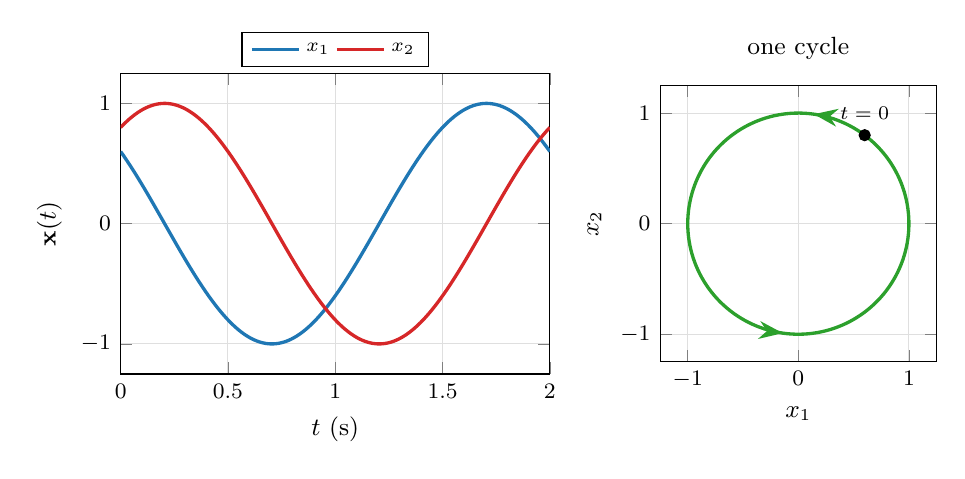
\begin{tikzpicture}
\begin{groupplot}[group style={group size=2 by 1, horizontal sep=1.4cm}, height=5.4cm]
\nextgroupplot[width=0.58\textwidth, xmin=0, xmax=2, ymin=-1.25, ymax=1.25,
  xlabel={$t$ (s)}, ylabel={$\mathbf x(t)$},
  legend style={at={(0.5,1.02)}, anchor=south}, legend columns=2, legend cell align=left]
  \addplot[cA, very thick, domain=0:2, samples=200] {0.6*cos(deg(pi*x)) - 0.8*sin(deg(pi*x))};
  \addplot[cD, very thick, domain=0:2, samples=200] {0.6*sin(deg(pi*x)) + 0.8*cos(deg(pi*x))};
  \legend{$x_1$, $x_2$}
\nextgroupplot[width=0.42\textwidth, xmin=-1.25, xmax=1.25, ymin=-1.25, ymax=1.25,
  axis equal image, xlabel={$x_1$}, ylabel={$x_2$}, title={one cycle}]
  \addplot[cC, very thick, domain=0:360, samples=160, postaction={decorate},
    decoration={markings, mark=at position 0.08 with {\arrow{Stealth[length=3mm]}},
                         mark=at position 0.58 with {\arrow{Stealth[length=3mm]}}}]
    ({0.6*cos(x) - 0.8*sin(x)}, {0.6*sin(x) + 0.8*cos(x)});
  \addplot[only marks, mark=*, black] coordinates {(0.6,0.8)};
  \node[font=\scriptsize, anchor=south] at (axis cs:0.6,0.85) {$t = 0$};
\end{groupplot}
\end{tikzpicture}
\end{center}
Four easy checkpoints, a quarter cycle apart: $(0.6, 0.8)$ at $t = 0$, $(-0.8, 0.6)$ at $t = 0.5$, $(-0.6, -0.8)$ at $t = 1$, $(0.8, -0.6)$ at $t = 1.5$.
\begin{marking}
1: both formulas, or the equivalent shifted sine and cosine of amplitude $1$. \ 0.5: period $2$ s. \ 0.5: the time plot starts at $0.6$ and $0.8$, with $x_1$ decreasing. \ 0.5: circle of radius $1$. \ 0.5: counter-clockwise.
\end{marking}

%=====================================================================
\section*{Question 5 \hfill (4)}

\ans{(a) [2]}
\[
x(t) = \begin{cases} 3t, & 0 \le t < 0.4,\\ 1.2, & t \ge 0.4. \end{cases}
\]
A straight ramp of slope $3$, ending at $1.2$, then a flat hold. The corner is at $t = 0.4$ s.
\begin{marking}
1: $3t$ on $[0, 0.4)$. \ 0.5: holds at $1.2$. \ 0.5: the sketch is a straight ramp, then flat.
\end{marking}

\ans{(b) [2]}
The two synapses disagree, so
\[
X = \frac{U}{s} + (\tau - \tin)\frac{U}{1 + s\tin}.
\]
The second term is $(\tau - \tin)$ times the input smoothed by the fast synapse. While the pulse is on, $u = 3$ and $\tin = 20$ ms is short, so the gap is
\[
(\tau - \tin)\,u = (0.1 - 0.02)\cdot 3 = \mathbf{0.24}.
\]
Just before $t = 0.4$ s the decoded value is about $1.2 + 0.24 = 1.44$, above the ideal ramp. When the pulse ends, $u = 0$ and the extra term dies within a few $\tin$. The stored integral is untouched, so $x$ settles at $\mathbf{1.2}$.
\begin{center}
\begin{tikzpicture}
\begin{groupplot}[group style={group size=1 by 2, vertical sep=0.35cm, xticklabels at=edge bottom},
  width=0.92\textwidth, xmin=0, xmax=1]
\nextgroupplot[height=2.6cm, ymin=-0.3, ymax=3.4, ylabel={$u(t)$}]
  \addplot[black, very thick] table[x=t, y=u] {pn3_data/q5_pulse.dat};
\nextgroupplot[height=6cm, ymin=-0.05, ymax=1.7, xlabel={$t$ (s)}, ylabel={$x(t)$},
  legend style={at={(0.5,-0.28)}, anchor=north}, legend cell align=left, legend columns=2]
  \addplot[black, very thick, dashed] table[x=t, y=ideal] {pn3_data/q5_pulse.dat};
  \addplot[cB, very thick] table[x=t, y=lead] {pn3_data/q5_pulse.dat};
  \addplot[cA, thick] table[x=t, y=spike] {pn3_data/q5_pulse.dat};
  \addplot[cC, thick] table[x=t, y=rate] {pn3_data/q5_pulse.dat};
  \legend{{ideal (a)}, {prediction: integral $+\,(\tau - \tin)(h_{\mathrm{in}} * u)$}, {Nengo LIF}, {Nengo LIFRate}}
  \draw[{Stealth}-{Stealth}, cD, thick] (axis cs:0.38,1.17) -- (axis cs:0.38,1.41);
  \node[cD, font=\scriptsize, anchor=west] at (axis cs:0.4,1.32) {$0.24$};
\end{groupplot}
\end{tikzpicture}
\end{center}
The spiking trace sits slightly under the prediction because the readout probe adds its own filter. The final value is still $1.2$.
\begin{marking}
1: the trace lies a constant gap above the ideal ramp while the pulse is on. \ 0.5: the gap is $0.24$ (accept $0.2$ to $0.25$). \ 0.5: after the pulse it returns to $1.2$.
\end{marking}
\begin{trap}
Reading the faster input synapse as a small delay. The error is an offset of size $(\tau - \tin)u = 0.24$, and it disappears once $u$ returns to $0$.
\end{trap}

%=====================================================================
\section*{Bonus Question 1 \hfill (2)}
Recurrent transform $A' = 0.98$ with $\tau = 0.1$ s and no input means
\[
A = \frac{A' - 1}{\tau} = \frac{-0.02}{0.1} = -0.2,
\qquad \dot x = -0.2\,x.
\]
The time constant is $\tau/(1 - A') = 0.1/0.02 = 5$ s, so $x(t) = e^{-t/5}$. It falls from $1$ to $0.5$ when $e^{-t/5} = 1/2$:
\[
t = 5\ln 2 \approx \mathbf{3.47}\ \text{s}.
\]
A recurrent gain $2\%$ below $1$ turns a perfect memory into a $5$ s leak. The same $2\%$ above $1$ would make the held value grow until it hit the radius.
\begin{center}
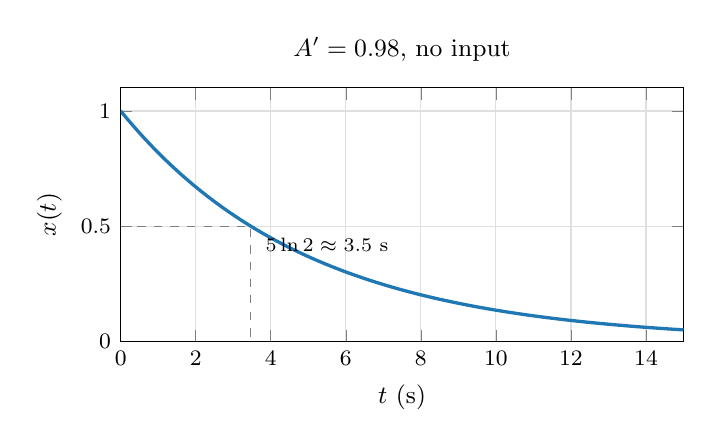
\begin{tikzpicture}
\begin{axis}[width=0.72\textwidth, height=4.8cm, xmin=0, xmax=15, ymin=0, ymax=1.1,
  xlabel={$t$ (s)}, ylabel={$x(t)$}, title={$A' = 0.98$, no input}]
  \addplot[cA, very thick, domain=0:15, samples=100] {exp(-x/5)};
  \draw[gray, dashed] (axis cs:0,0.5) -- (axis cs:3.47,0.5) -- (axis cs:3.47,0);
  \node[font=\scriptsize, anchor=west] at (axis cs:3.6,0.42) {$5\ln 2 \approx 3.5$ s};
\end{axis}
\end{tikzpicture}
\end{center}
\begin{marking}
1: $\dot x = -0.2x$, or a leak with time constant $5$ s. \ 1: about $3.5$ s to fall from $1$ to $0.5$, with a decaying sketch.
\end{marking}

\end{document}
